\newpage
%%%%%%%%%%%%%%%%%%%%%%%%%%%%%%%%%%%%%%%%%%%%%%%%%%%%%%%%%%%%%%%%
%%%%%%%%%%%%%%%%%%%%%%%%%%%%%%%%%%%%%%%%%%%%%%%%%%%%%%%%%%%%%%%%
%%%%%%%%%%%%%%%%%%%%%%%%%% Enunciado %%%%%%%%%%%%%%%%%%%%%%%%%%%

\begin{myblock}
\phantomsection\addcontentsline{toc}{section}{Ejercicio \#2 | Redes Neuronales Multicapa}
\section*{Ejercicio \#2 | Redes Neuronales Multicapa}

Considera las redes multicapa (con funciones de activación lineal), 
que se muesstran en la figura \ref{fig:redA_redB}:

\begin{itemize}
    \item Describe una ventaja (al menos) de la red A sobre la red B.
    \item Describe una ventaja (al menos) de la red B sobre la red A.
\end{itemize}

\end{myblock}

%%%%%%%%%%%%%%%%%%%%%%%%%%%%%%%%%%%%%%%%%%%%%%%%%%%%%%%%%%%%%%%%
%%%%%%%%%%%%%%%%%%%%%%%%%%%%%%%%%%%%%%%%%%%%%%%%%%%%%%%%%%%%%%%%

\begin{figure}[h!]
    \centering
    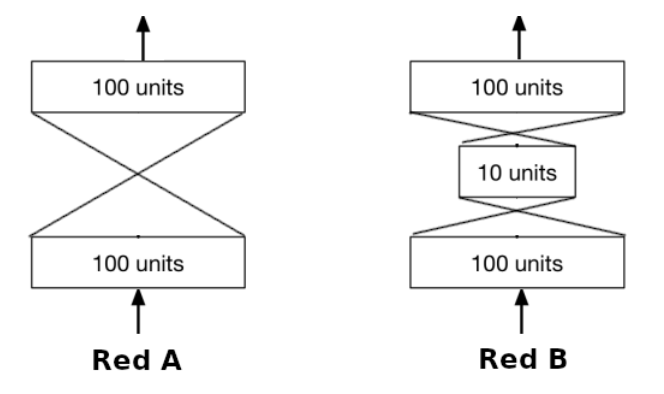
\includegraphics[width=0.8\linewidth]{Images/redA-redB.png}
    \caption{Esquema de dos redes neuronales.}
    \label{fig:redA_redB}
\end{figure}


%%%%%%%%%%%%%%%%%%%%%%%%%%%%%%%%%%%%%%%%%%%%%%%%%%%%%%%%%%%%%%%%
%%%%%%%%%%%%%%%%%%%%%%%%%%%%%%%%%%%%%%%%%%%%%%%%%%%%%%%%%%%%%%%%

\subsection{Ventajas de la Red A}

% La principal ventaja de la Red A es que, al estar trabajando con funciones de activación lineal, aprende
% cualquier mapeo, valga la redundancia, lineal. Esto le permite preservar por completo la información
% original de lo que sea que estemos haciendo pasar por la red: imágenes, texto, tablas, etc. Creo que lo 
% más importante es que intenta replicar a la perfección los datos, para tareas donde los detalles son de 
% suma importancia.

% Sin embargo, también esto es una desventaja. Al pasar la información de manera directa, de los 100 nodos
% a los otros 100 nodos, se corre el riesgo de sobreajustar el entrenamiento a nuestros datos y no llegar a 
% generalizar en absoluto. 

Nuestra Red A es esencialmente una transformación lineal completa entre dos espacios de dimensión 100. Hay 
que tomar en cuenta que la actiavición de nuestras capas son lineales, por lo que la red puede representar
cualquier transformación lineal entre entrada y salida en el mismo espacio. Lo anterior provoca que no se
pierda información o detalles de las características de nuestros vectores de entrada. 

Sin embargo, la Red A tiene una desventaja bastante crítica para la mayoría de las tareas. Al pasar la 
información de manera directa, de los 100 nodos a los otros 100 nodos, se corre el riesgo de sobreajustar
el entrenamiento a nuestros datos y no llegar a generalizar en absoluto. 

\subsection{Ventajas de la Red B}

% Para el caso de la Red B, tenemos una arquitectura muy similar a la de la Red A, aunque en medio de las
% dos capas de activación (de 100 neuronas cada una), hay un cuello de botella de 10 neuronas. Este hecho
% obliga a la red a aprender características que le permitan generalizar mejor. De esa manera se vuelve un
% poco más robusta al ruido y mitiga un poco el sobreajuste. 

% Podríamos pensar en una tarea sencilla, como la de eliminar ruido. Si intentamos extraer las características
% más generales de nuestro corpus, tener al menos una capa oculta que funcione de cuello de botella, tendremos
% la posibilidad de comprimir esos datos y eliminar ruido, algo que no sucedería en la Red A, pues se pasan
% los datos de manera directa. 

% Justo el mencionado cuello de botella mitiga un poco el sobreajuste de la Red A, pues al reducir dimensionalidad
% está trabajando también como regularizador. Nuestro algoritmo de optimización se enfocará en comparar las 
% reconstrucciones y quedarse con aquellas que mejoren la salida, descartando aquellas en las que tengamos 
% salidas con ruido aumentado, en lugar de filtrado. 

Ahora bien, la Red B introduce un cuello de botella de 10 neuronas entre capas de dimensión 100. Esto provoca
un efecto de regularización, pues al reducir la dimensionalidad en dicha capa intermedia, se fuerza al modelo
a aprender representaciones latentes comprimidas que capturen las características más importantes de nuestros
datos, Podríamos pensar en que tal efecto es similar al de una proyección de Análisis de Componetes Principales (PCA)
, en donde el cuello de botella concentra la mayor varianza explicativa de nuestros datos. 

Justo esa arquitectura con una capa en medio es lo que vuelve a la Red B a una más robusta en términos de
generalización. A diferencia de la Red A, esta corre menos riesgo de sobreajustar ya que no pasa de manera
directa los datos de la capa de 100 nodos a la otra de 100 nodos. El modelo se queda con un ``mapeo de características''
reteniendo los patrones estructurales de nuestros datos. Claro que con sus limitaciones, pues después de todo 
se trata de una red sencilla. 

Matemáticamente, esto se vería algo así:

\[
    \text{La Red B se implementa como:} \;\;\;\;\; f(x) = W_2 W_1 x
\]

En este caso:

\begin{itemize}
    \item $W_1 \in \mathbb{R}^{10 \times 100}$ y proyecta $x$ a un subespacio de dimensión 10.
    \item $W_2 \in \mathbb{R}^{100 \times 10}$ reconstruye desde el anterior subespacio a dimensión 100. 
\end{itemize}

Por lo tanto, la matriz de la red se representaría de la siguiente manera:

\[
    M_{\text{Red B}} = W_2 W_1 \in \mathbb{R}^{100 \times 100} 
\]

Y esto implica que: 

\[
    \rank(M) \leq \min\{\rank(W_1), \rank(W_2)\} \leq 10
\]

La primera transformación $W_1$ crea un espacio intermedio cuya dimensión es como máximo de 10. La segunda
transformación $W_2$ actúa sobre el espacio anterior, ya de por sí limitado. Por lo que la dimensión
del espacio final no puede ser mayor que la del cuello de botella. Esto lleva a que $\rank(W_2 W_1) \le \rank(W_1)$. 
Creo que con lo anterior queda demostrado que la Red B no puede representar cualquier transformación lienal 
arbitaria en $\mathbb{R}^{100}$, solo aquellas de rango bajo, i.e. 10. 

Podemos pensar en la tarea de filtrado de ruido en audio o imágenes, o detección de bordes. El cuello de botella
va a favorecer la extracción de propiedades generales en lugar de detalles específicos que sometan a nuestro
modelo a sobreajustar. 

\clearpage










